\documentclass{main}
\begin{document}
\section{Invisible Internet Project - I2P}
This is a project trying to implement \textbf{Garlic Routing} - A Routing protocol built over onion routing.
It is not used widely as of today because it needs slightly more technical knowledge to set up for
the first time for use. Also, the sites outside the network of invisible internet cannot be accessed
through the invisible internet. One may access outside internet through proxies (which do exist) but 
the proxies may be malicious and it may not be safe to do so. This also is a big problem hindering the
popularity of i2p.

\subsection{I2P Protocol}
I2P adds more layers in Application Layer of primitive internet to introduce anonymity. Figure \ref{fig:i2p_protocol_stack}
shows the layers in this stack.

\begin{figure}[h]
	\centering
	\caption{I2P Protocol Stack}
	\label{fig:i2p_protocol_stack}
	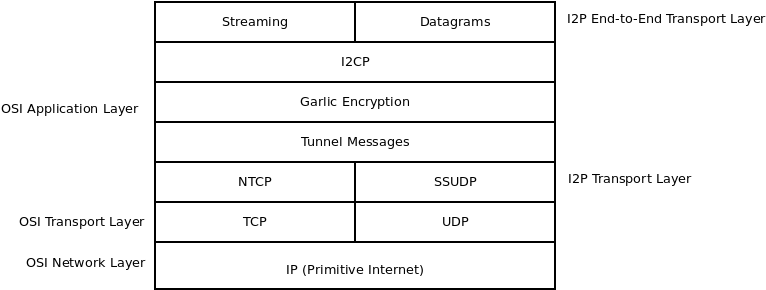
\includegraphics[width=\textwidth]{Resources/images/i2p_protocol_stack.png}
\end{figure}

I2P transport layer is built over Transport layer of regular internet. It is strictly for next-hop transfer
among I2P routers. This is non-anonymous transfer. This layer has two protocols built over TCP and UDP each.
\begin{itemize}
	\item NTCP2 - New I/O based TCP
	\item SSU - Secure and Semi-Reliable UDP
\end{itemize}

\subsection{Structure of I2P: Components}
\begin{itemize}
	\item \textbf{Tunnel} \\
		Messages are sent from one node to another through tunnels. There are two tunnels, outbound tunnel
		and inbound tunnel. This is needed as per Garlic Routing protocol. The sender first builds an 
		outbound tunnel. It gets the details of Inbound tunnel from netDB. \\
		In a tunnel a gateway refers to first router and the last router is called endpoint.
		A user might have multiple such outbound and inbound tunnels. These tunnels
		used in I2P are \textbf{unidirectional} as opposed to bi-directional routes in Tor. \\
		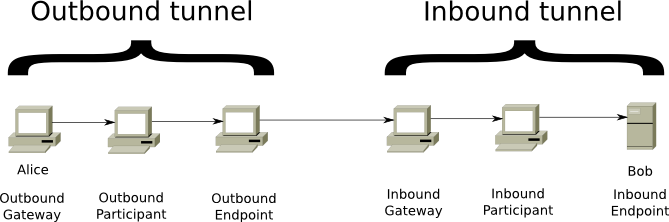
\includegraphics[width=0.95\textwidth]{Resources/images/i2p-tunnels.png}

		The sender adds routing instructions with the message, encrypts it and sends it through the tunnel.
		Just like Onion routing, this message is also encrypted using layered encryption. When the endpoint
		recieves the final message, it gets the routing instruction to the inbound gateway of reciever.
		The inbound gateway then sends this message to inbound endpoint through the tunnel. Except for this 
		difference, if we see tunnels as gateway to endpoint, both work in a similar way.

		Gateway accumulates some messages to be sent through the tunnel, adds path to reciever and
		converts them to \textbf{Garlic Message} so that they can be sent through tunnel.
		When the endpoint of tunnel finally decrypts the message, it separates the messages and forwards them 
		to the required hosts.
	\item \textbf{Network DataBase} \\
		Network Database stores the information about the routers present in the network. It also stores information
		about the tunnel gateways for inbound tunnels of users. In I2P, routers are identified by their public keys.
		This Network Database is a decentralized database. \\
		When a user wants to communicate with some other router in the Invisible Internet, he needs to lookup in the
		network database to find the details of inbound tunnel gateway for reciever. As it is a decentralized database,
		possibly, a router may not have access to complete database at any given time. As I2P is not widely used, it 
		is possible to find these details in a few tries but if the usage increases, it might become difficult to access
		this information.\\
		Network database stores two kinds of data: \textbf{leaseSets}(Section \ref{subsubsec:leaseSet}) and \textbf{routerInfo}(Section \ref{subsubsec:routerInfo})

\end{itemize}
\subsection{Network Database}

\subsubsection{Distributed Storage}
Network Database (NetDB) is a distributed storage. The storage is distributed among I2P nodes.
A special set of nodes called \textbf{floodfill} nodes are used for storing the data. There is no fixed
set of floodfill nodes. The users of I2P can Opt-in as Floodfill routers. Any router which wants to 
publish it's routerInfo does so by sending the data to the nearest floodfill router. The information of
whether a router is a floodfill router is stored in routerInfo of the corresponding router. When a floodfill
router gets a DatabaseStoreMessage, it floods it.

For flooding, it looks up several floodfill routers closest to the routing key of NetDb entry, where routing
key is SHA256 hash of routerIdentity/Destination with date appended.

Unlike Tor, these floodfill peers need not be trusted, and may change over time. Usually, the floodfill
routers are one with large bandwidth availability. The only extra work they need to do is \textbf{respond to
netDB stores and queries}.

\subsubsection{Lease Sets}
\label{subsubsec:leaseSet}
Lease Sets are used to document tunnel entry points for a particular client destination. The following information is
stored in a Lease Set.
\begin{description}
	\item [Lease] stores information of the inbound tunnel gateway. A lease
		stores the following information. It is needed to send messages to the Destination.
		\begin{description}
			\item [Gateway Router] is specified for the tunnel. It is specified by spcifying it's identity.
			\item [Tunnel ID] to be used to send message through the tunnel.
			\item [Expiry Date] stores the time till when the tunnel is available.
		\end{description}
	\item [Destination] encryption key, signing key and a certificate.
	\item [Additional encryption public key] for use in encrypting garlic messages. It is used for end-to-end 
		ElGamal/AES + Session Tag encryption.
	\item [Signature] of the lease set to ensure that the data is published by the entity mentioned
		in destination.
\end{description}
There are various types of Lease sets like Unpublished Lease sets, Encrypted LeaseSets etc.

\subsubsection{Router Info}
\label{subsubsec:routerInfo}
RouterInfo includes the following details
\begin{description}
	\item [Router's Identity] stores an encryption key, a signing key and a certificate to authorize that.
		The public\_key is used for ElGamal Encryption in next-hop messages. The signing public key and
		key certificate are used for verifying signatures.
	\item [Contact Addresses] where the router can be reached. It contains mapping of transport protocol (NTCP or SSU)
		with ip address and port. 
	\item [Publish Date] is the time when this info was published.
	\item [Options] is a set of arbitrary options for telling the bandwidth capacities, router version, netId. There
		are some other stat options also.
	\item [Signature] of all the above data.
\end{description}
Router Info is stored in NetDB. This is required for building tunnels.

\subsection{Tunnels}
Tunnels can be divided into two types of tunnels, namely inbound tunnels and outbound tunnels. The creator of the
tunnel is the only one who knows all participants of tunnels. There are three types of routers in tunnels, namely
gateway, participants, and endpoint. The gateway collects all messages, combines them and sends to next hop. The
participant routers just decrypt/encrypt and forward to nexthop. They don't even know if it is an inbound or outbound
tunnel. The endpoint recieves the messages, opens it and forwards it, either to another router, or to a tunnel gateway
or locally.

\subsubsection*{Building a Tunnel}
For building a tunnel, we need to ensure that the hops can't be associated to each other. Only the next hop peers
should be able to know that they are in same tunnel. Every hop in the tunnel gets a random non-zero tunnel ID. Every
record gets a random tunnel IV key, reply IV, layer key and reply key. The record contains the tunnel ID, the next
hop tunnel ID, routerid hash, tunnel layer key and iv key, reply key and iv and some uninterpreted padding to send to next hop.
The tunnel creation is accomplished by a single message passed along the path of peers in the tunnel, rewritten
in place, and transmitted back to the tunnel creator. This is made up of variable number of records, each record
potentially for each peer along the path. For building an inbound tunnel, an outbound tunnel is used to send this message
whereas it is directly sent as next hop for building outbound tunnel. Every hop replaces it's record by it's reply and
the endpoint is instructed to send the message to the tunnel creator.

A gateway first does some message pre-processing and then sends it the next hop after gateway encryption. In this pre-processing,
it takes the collected I2NP messages, makes \{delivery instructions,message\} pairs, adds tunnel ID, IV, checksum and padding. It
then picks an IV, iteratively encrypts it and the message as needed and forwards that to next hop with tunnel ID and IV.

When a participant recieves a tunnel message, it reads the tunnel
id, maps it with next hop tunnel id and sends it to the next hop. The participant encrypts the recieved IV with AES256ECB
using their IV key to determine the current IV and uses that IV with it's layer key to encrypt that data. It then encrypts 
the current IV with AES256/ECB using their IV key again, then forwards the tuple \{nextTunnelId,nextIV,encryptedData\} to the
next hop.

For an outbound tunnel, the gateway just encrypts data using it's layer key to get the pre-processed data. Whereas for inbound
tunnels, the endpoint needs to decrypt that according to each hop's layer key and IV to get the pre-processed data.
\subsection{Sending Messages}
For sending a message, a router needs an outbound tunnel. For this, a tunnel is created. For creating a tunnel, the
router requests routerInfo from netDB through Database. It selects routers to use in the tunnel and builds a tunnel.
Then it uses this outbound tunnel to request leaseSet of destination from Database. This leaseSet is used to get 
the inbound tunnel gateway routerIdentity. It then puts delivery instruction for the message as this gateway router's
information and tunnel id. This is then encrypted accordingly and sent to next hop. When it reaches the endpoint of this
tunnel, it gets the forwarding instructions. The message is forwarded to the gateway which then sends it to the required 
destination. For a reply, the sender needs to put it's lease or Destination information in the message sent.
\end{document}
